\documentclass{article}
\usepackage[portuguese]{babel}
\usepackage[utf8]{inputenc}
\usepackage[T1]{fontenc}
\usepackage{graphicx}
\graphicspath{{c:/images/} }
\usepackage[margin=0.7in]{geometry}

\usepackage{fancyhdr}

\pagestyle{fancy}
\fancyhf{}
\rhead{Sistemas Computacionais Embebidos}
\lhead{Sistema de Monitorização e Alarme (1ªParte)}
\rfoot{Página \thepage}

\begin{document}

	\title{\textbf{Sistema de Monitorização e Alarme (1ªParte)} \\ \large Sistemas Computacionais Embebidos - 1º Trabalho de Laboratório \\ \large 2º Semestre 2014/2015}
	%\title{\textbf{Sistema de Monitorização e Alarme (1ªParte)}}
	
	\author{Grupo n.º 3: Margarida Reis(73099) - Sofia Silva(73483) - Tiago Ricardo(73649)}
	
	\maketitle	
	
	
	\section{Estruturas de Dados}
	Como forma de disponibilizar as funções pedidas no enunciado do projecto, recorreu-se às seguintes estruturas de dados:
	
	\subsection{Relógio}		
	
		
		O relógio é construído com base num dos temporizadores do PIC e fornece uma série de funções ao utilizador que permitem verificar a hora corrente, definir um alarme para as horas e acertar a hora. O relógio permite também monitorizar o "estado do sistema", através da inspecção periódica dos valores dos sensores.
		
	\begin{center}
		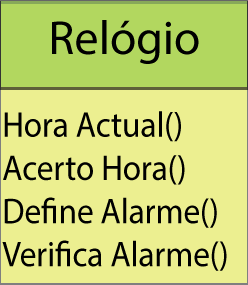
\includegraphics[width=0.10\textwidth]{scereport_01}
	\end{center}
	

	
	
	\subsection{LCD e Besouro}		
	
	O LCD é utilizado na interface do utilizador, para que este possa verificar a hora atual, os valores lidos pelos sensores, as alterações e os alarmes no modo de modificação. Numa situação de alarme, o utilizador é notificado no LCD. O Besouro é também utilizado na interface do utilizador na notificação de uma situação de alarme através de um sinal sonoro. 
	
	\begin{center}
		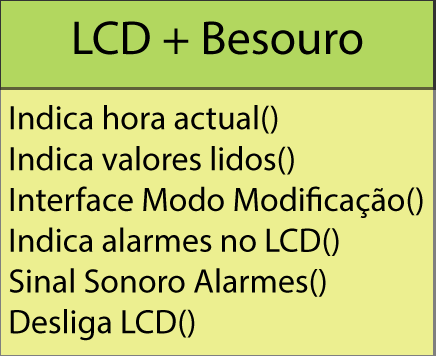
\includegraphics[width=0.15\textwidth]{scereport_05}
	\end{center}
	
	
	
	
	\subsection{Botões S2/S3}		
	

	O botão S3 está associado a uma interrupção que permite ao utilizador entrar no modo de modificação, desligar os alarmes, sair do modo de poupança de energia e entrar no modo de modificação. Para além disto, o botão S3 é utilizado como auxiliar na navegação do cursor no LCD no modo de modificação, permitindo selecionar um dos campos. O botão S2 é utilizado para alterar os valores em cada campo do modo de modificação.
		
		\begin{center}
			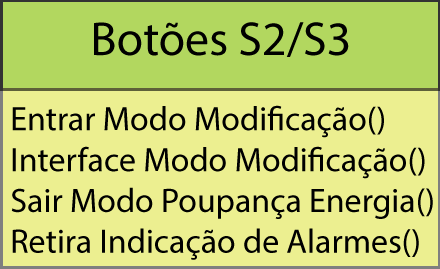
\includegraphics[width=0.15\textwidth]{scereport_06}
		\end{center}
		
	
		\subsection{Sensores de Luminosidade e Temperatura}		
		
		\begin{center}
			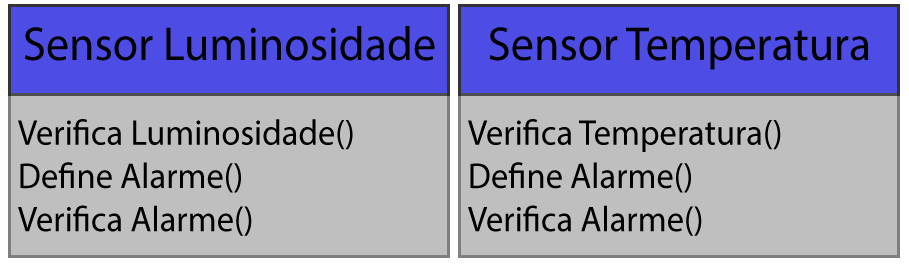
\includegraphics[width=0.3\textwidth]{scereport1_03}
		\end{center}
		
		\subsection{Memórias EEPROM}		
		Existem duas memórias EEPROM, uma externa e outra interna com funções distintas que passam a ser descritas de seguida.
		\subsubsection{Memória EEPROM Externa}
		Na EEPROM externa é guardado um registo histórico dos eventos mais recentes e a informação necessária à gestão desta. O registo dos eventos tem em conta a estampilha temporal, o código destes e os parâmetros que caracterizam os mesmos. 
		\begin{center}
			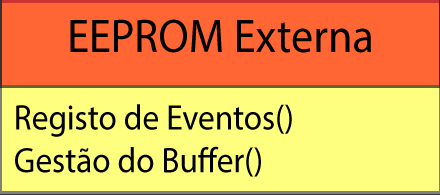
\includegraphics[width=0.15\textwidth]{scereport_03}
		\end{center}
		\subsubsection{Memória EEPROM Interna}
		Na EEPROM interna são mantidos atualizados os parâmetros relevantes ao correto funcionamento do sistema (alarmes, PMON, TSOM, NREG e relógio), para que possam ser recuperados em situações em que se interrompa a alimentação ou seja feito um \textit{reset}.
		
	
		\begin{center}
			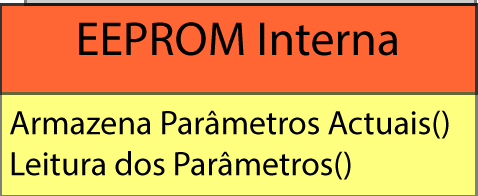
\includegraphics[width=0.15\textwidth]{scereport_14}
		\end{center}
		
		\section{Decisões de Projecto}
		Nesta secção apresentam-se as decisões tomadas pelo grupo durante a elaboração do projecto:
		
		\begin{itemize}
		\item Não disparam alarmes durante o modo de modificação;
		\item Se disparar um alarme a letra correspondente a esse alarme (A, T ou L) fica escrita no LCD até haver interacção do utilizador, ou seja, quando é pressionado o botão S3.
		\item No modo de modificação, o valor do alarme das horas só é apresentado a partir do momento em que o cursor se encontra sobre a letra A;
		\item Na rotina principal, considerou-se a seguinte sequência de operações:
		
			\subitem -Rotina de Verificação de Alarmes;
			\subitem -Modo de Modificação;
			\subitem -Aviso de Alarmes;
			\subitem -Rotina de leitura dos sensores (de acordo com o período indicado pela variável PMON).
		\item Para cada tipo de alarme, o sinal sonoro emitido pelo besouro tem uma frequência diferente; 
		\item No modo de modificação, o utilizador pode pressionar de forma continuada o botão S2, se preferir, para alterar os valores dos parâmetros;
		\item Sempre que possível o sistema entra em modo \textit{sleep} e sai desse modo quando ocorre uma interrupção do \textit{timer} ou do botão S3;
		\item A verificação dos alarmes é feita segundo a segundo;
		\item Memória Interna:
			\subitem Os valores da memória interna são recuperados se forem coerentes. Para verificar a coerência dos valores recorre-se a um valor armazenado na posição de memória 0x0B, a "palavra-mágica". Este valor é calculado através da leitura de todas as posições de memória anteriores, excepto a dos segundos. Este valor não é lido porque só se escreve na posição de memória alocada para os segundos quando há uma falha de alimentação e quando isso ocorre verificou-se que não há tempo para calcular a ``palavra-mágica'' correspondente, sendo a verificação da coerência dos segundos feita à parte. 
			
			Assim, quando é escrito um bloco na memória interna, calcula-se a ``palavra-mágica'' desse bloco e actualiza-se depois o valor da ``palavra-mágica'' global que corresponde à soma das ``palavra-mágicas'' de todos os blocos - bloco da hora do alarme (3 \textit{bytes}), bloco dos parâmetros (PMON, TSOM e NREG - 3 \textit{bytes}), bloco da luminosidade (1 \textit{byte}), bloco da temperatura (1 \textit{byte}), bloco das horas (1 \textit{byte}) e bloco dos minutos (1 \textit{byte}.)
			
			Quando o programa inicia lê-se a posição de memória que armazena a ``palavra-mágica'' e compara-se esse valor com o \textit{checksum}. O \textit{checksum} é calculado somando o valor armazenado em todas as posições de memória antes de 0x0B, excluindo a dos segundos. Se os valores forem iguais significa que os dados armazenados na memória interna são coerentes e podem ser carregados para o programa. Se os valores não estiverem coerentes são carregados os valores por omissão.
		\item LVD:
			\subitem Verificou-se que só existe tempo para escrever um \textit{byte} na memória interna a partir do momento em que existe uma falha de alimentação. Assim, tomou-se a decisão de guardar os minutos e as horas sempre que são atualizados e os segundos apenas quando há uma falha de alimentação. Como só se tem tempo para escrever um \textit{byte}, não se pode guardar a ``palavra-mágica'' actualizada deste bloco, motivo pelo qual a verificação da coerência deste valor é feita à parte. No início do programa, lê-se a posição de memória que contém os segundos e se o valor lá armazenado estiver entre 0 e 59 assume-se que é coerente.
			Relativamente ao ocorrer um \textit{reset} o sistema acede aos segundos guardados antes do último \textit{power down}.
		\end{itemize}
		
		\section{Fluxograma do Projeto}
		\begin{center}
			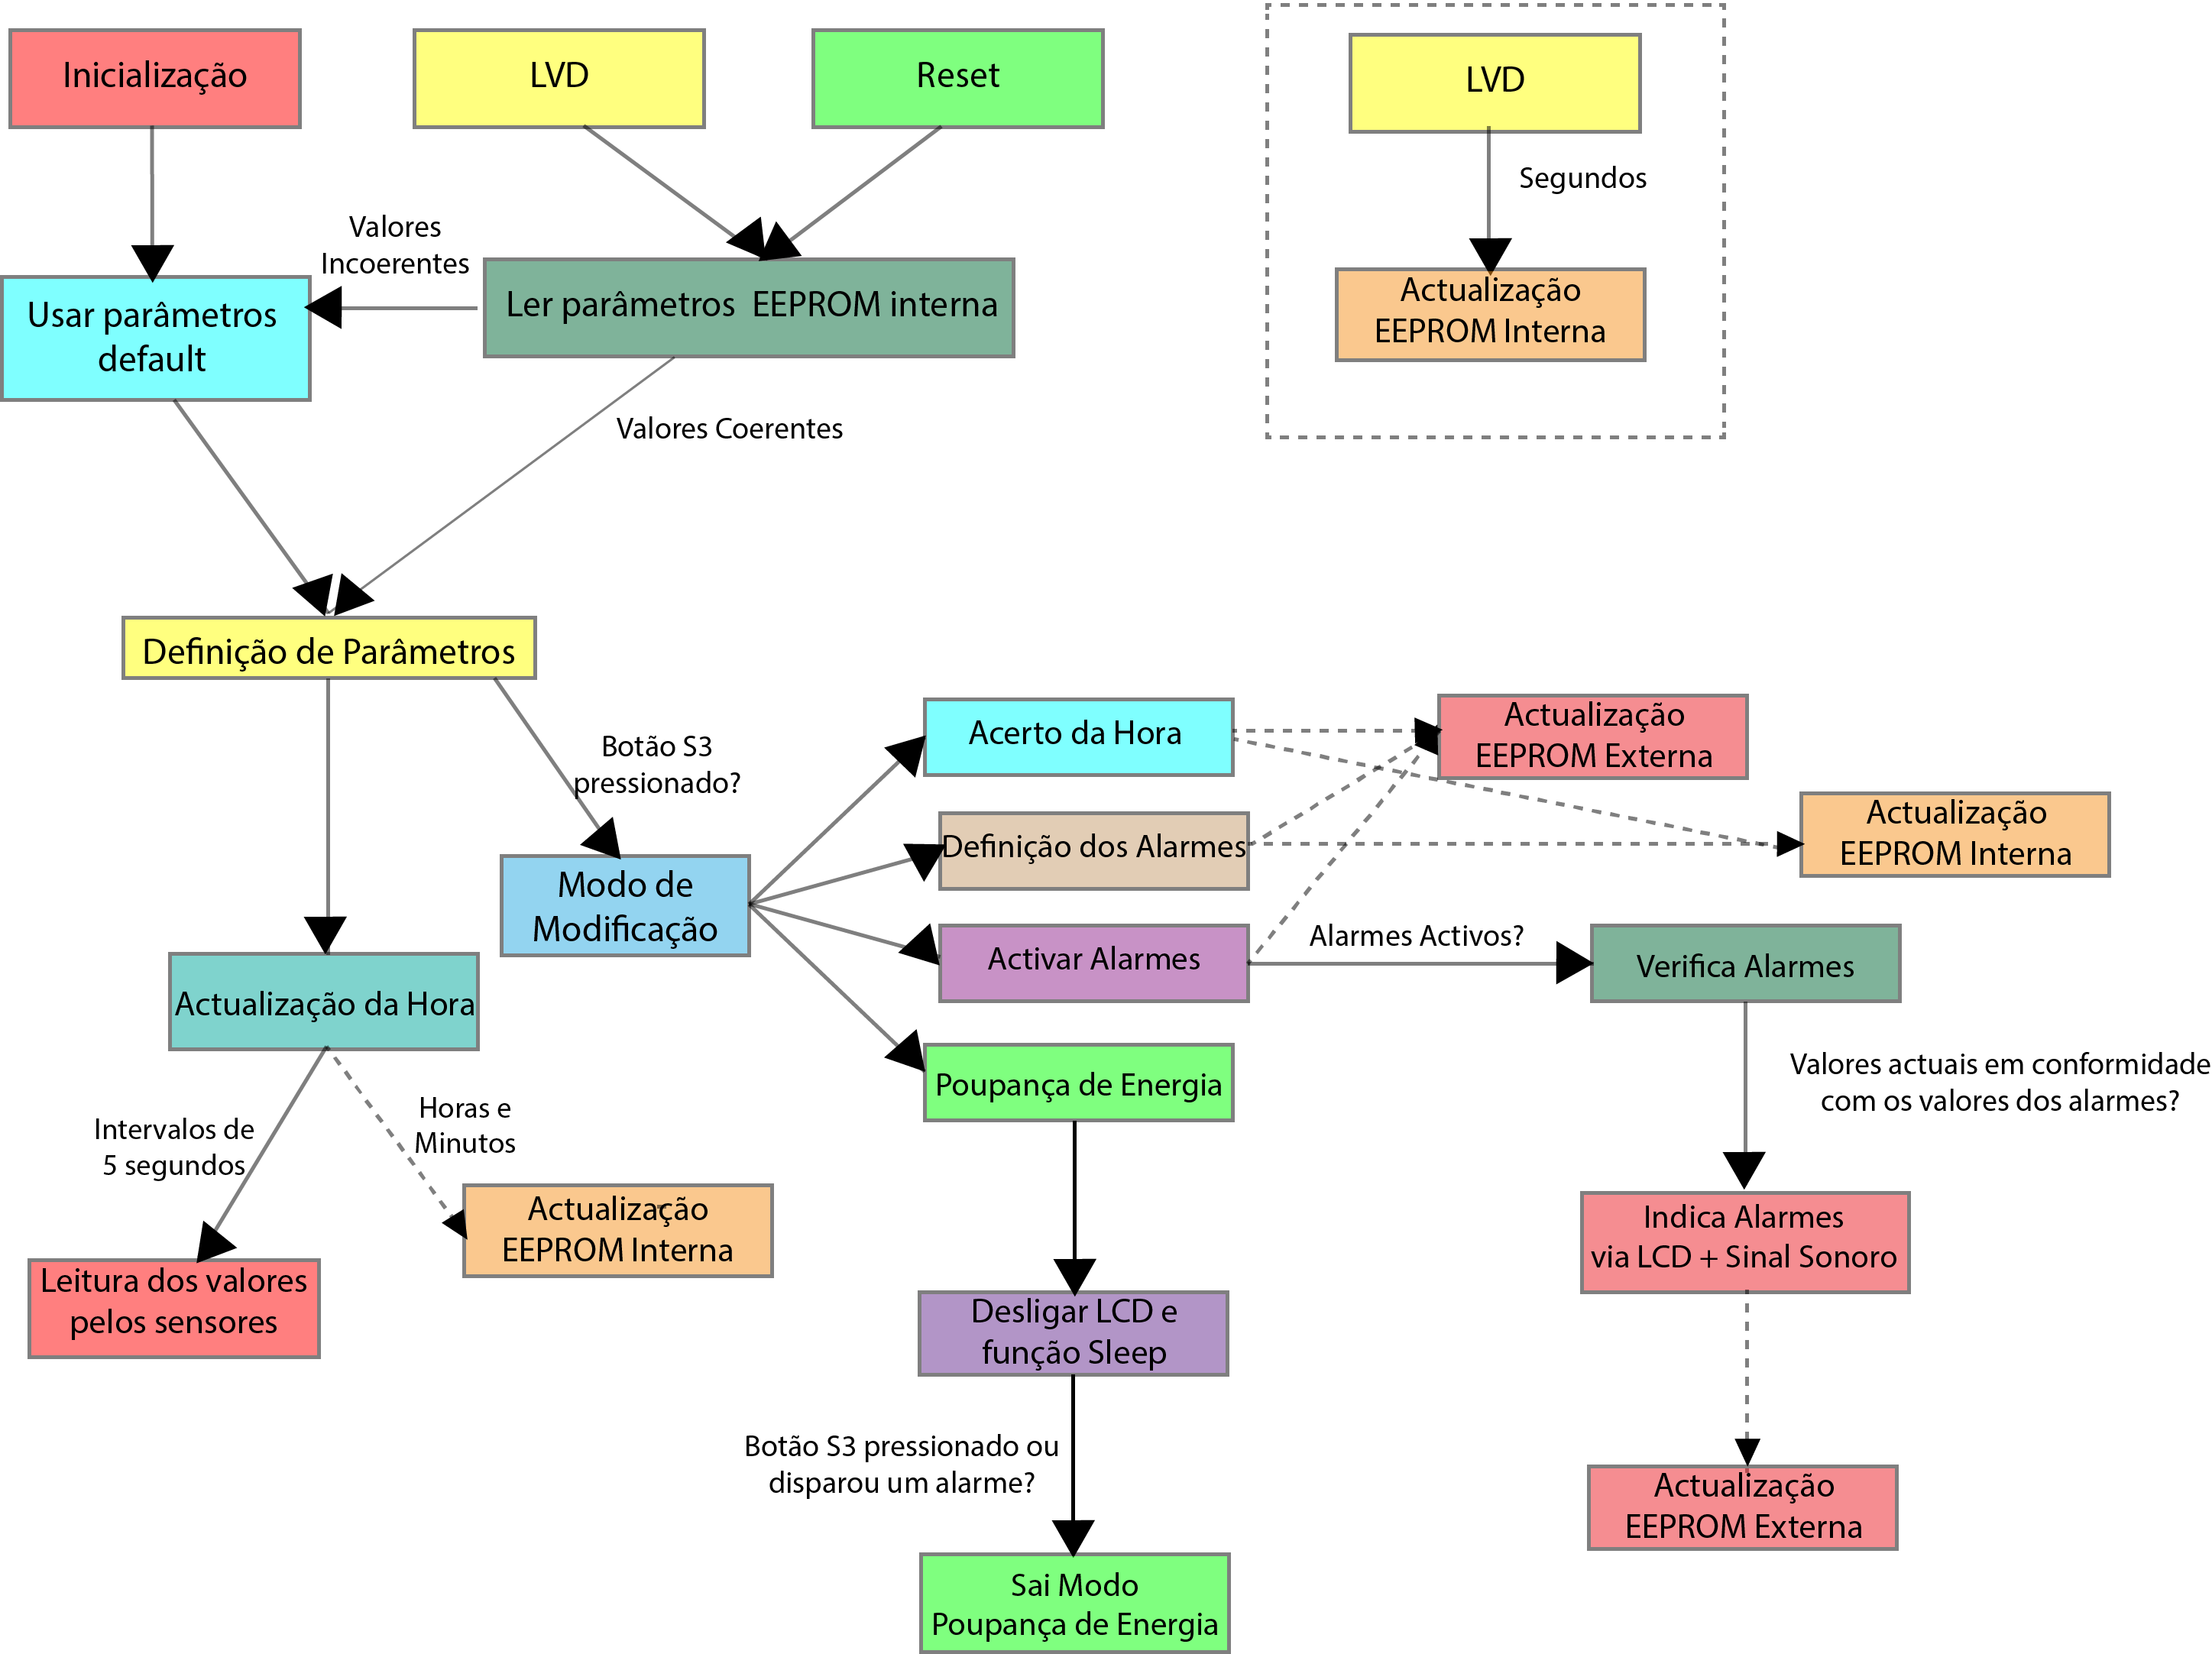
\includegraphics[width=1\textwidth]{scemaqestados}
		\end{center}
		
	
\end{document}